\chapter{People Recognition} \label{cha:recognition}
The goal of this chapter is to shows which types of techniques could be used to understand, given two images of a human, if the represented person is the same or not.

\section{Problem definition}
The \textbf{people recognition module}, also known as the \textbf{people identifier module}, overall the entire project as the role of connecting in a consistent way the two remaining modules, the detector and the tracker. The tracker works for the majority of the time, following the \textbf{main subject}, called \textbf{leader}. Then, when it fails or after a certain amout of time, the detector locates all the people in the incoming frame. Finally, the recognizer has to answer a simple question:
\begin{tcolorbox}
	\begin{center}
		\underline{\textit{Is this person the leader?}}\\
		Formally, given an image, cropped on the bounding box of a person, and a set of other images, with the same characteristics, containing various people labelled with names. Choose which is the name of the unknown person.
	\end{center}
\end{tcolorbox}
In our specific scenario, we are interested only into understanding if a bounding box contains a representation of the leader or not. For this reason the label can be considered with only two values: "\textit{positive}" or "\textit{negative}", "\textit{leader}" or "\textit{other}".\\

\subsection{Video surveillance application}
This challenge is extremely important in the video surveillance field. In fact, one of the most common application is to reconstruct where a person was seen during a certain time slot. The video surveillance application is a little bit different from the one in which we are interested:
\begin{tcolorbox}
	\begin{center}
		Given a dataset of images of people, and given as request a query containing an unknown image of a person, extract from the dataset all the images that contain the same person of the query.
	\end{center}
\end{tcolorbox}
From a high-level point of view, the two problems might look different but essentially are the same. The key idea is to look for all the images that might contain the person of the query. Then, according to the task, retrieve this list of people or use them and all the associated information to understand who is the person of the query.\\
Another difference comes from the acquisition of images. In our scenario, the webcam is mounted on the robot that is moving around, while in video surveillance the cameras are often static but multiple of them can simultaneously collect frames. We took inspiration from both single-camera scenarios\cite{reID_withSSN} and multi-camera systems\cite{multiFeatures_reID}.


\section{Not working methods}
This section is focused on some unsuccessful technique was explored during the development of the general structure for the project.

\subsection{Offline algorithms}
An offline algorithm (explained in~\Cref{sec:goturn}) is a great choice for training methods able to judge situations quickly. In this case, we have considered an \textbf{SVM (Support Vector Machine) classifier}.\\
This method is a supervised learning model based on a linear separator. The essential idea is to find the line\footnote{A line in 2D problems, that is converted into a hyperplane in N-dimensional scenarios.} that divide the dataset into two sections where respectively the two classes of interest lie (a visual representation is given in~\Cref{fig:howItWorks_svm}). The method could work if each image of a person is converted into a point, as explained in~\Cref{sec:classifiers}.\\
But this approach has a ground truth problem. The offline methods require prior knowledge of the context of application to train ad hoc models. In our case, the element to know is "\textit{Who is the leader?}". Based on this information the dataset can be split into two classes, the images representing the leader and the other ones, then the SVM classifier can be trained. The result is a model that always recognise one person, exactly the same person all the times.\\
Unluckily, this prior knowledge is not given. The algorithm should recognise all types of people after seeing them for a few seconds. This is the context where an online algorithm can be wisely used.
\begin{figure}
	\centering
	\begin{minipage}{.59\textwidth}
		\centering
		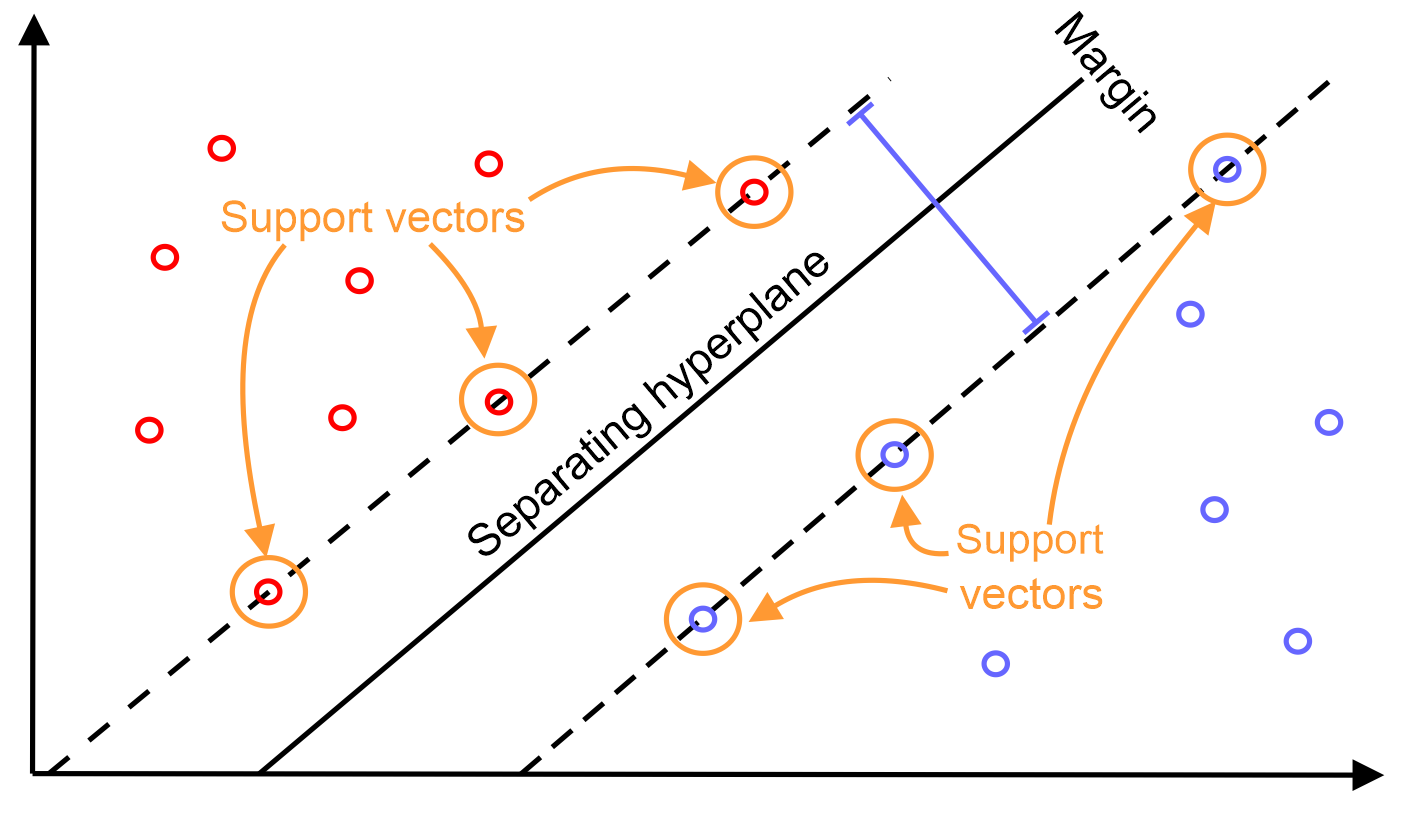
\includegraphics[width=1\linewidth]{images/recognition/howItWorks_svm}
		\captionof{figure}{The overall mechanics of SVM. The red and blue classes are divided by the hyperplane that maximizes the margin length, defined as the shortest distance from the closest point on both sides.}
		\label{fig:howItWorks_svm}
	\end{minipage}
	\begin{minipage}{.39\textwidth}
		\centering
		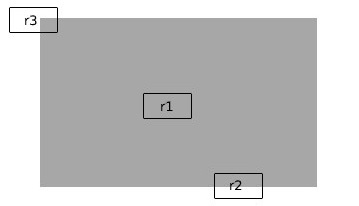
\includegraphics[width=1\linewidth]{images/recognition/kpMatch_regions}
		\captionsetup{margin=0.5cm}
		\captionof{figure}{Three possible regions that can be used as keypoints. R1 cover a complete flat region. R2 is located on an edge. R3 is placed on a corner, this is the location that can be better recognised.}
		\label{fig:kpMatch_regions}
	\end{minipage}
\end{figure}

\subsection{Key points matching}
The key points, or \textbf{feature points}, matching is a technique that compares two images and tries to recognise which are the common elements of the two. It is widely used to find small patterns in complex images, understand the variation of orientation, stitching panorama view and judge if the subject of two pictures could be the same.\\
This technique is based on key points. These elements are position in the image that can be easily located and identified as unique. In~\Cref{fig:kpMatch_regions} are shown three regions, a flat area, an edge and a corner. The most recognizable point is the one placed at the corner. If an object appears in two images a key point should be recognised in both the appearances.

\subsubsection*{Technique definition and known algorithms}
This technique is divided into two modules:
\begin{itemize}
	\item \textbf{Feature localization}: This module working on a single image at a time, is internally divided into:
	\begin{itemize}
		\item \textbf{Feature detection}: Given the raw image the goal is to identify all the corners that can be easily re-identified in another image.
		\item \textbf{Feature description}: A small area containing few pixels cannot be easily matched. So, the descriptor needs to take each identified key point and normalize them in order to be independent respect to the image conditions like illumination and orientation. This key point enriched with additional information is the feature point.
	\end{itemize}
	A visualization of the feature localization is shown in~\Cref{fig:kpMatch_tesla}.\\
	To solve this task exist several methods were used\footnote{Note that since the mechanics of the methods are similar and this technique has not actually been implemented in the thesis the algorithms reported here are not explained.}:
	\begin{itemize}
		\item \underline{SIFT (Scale-Invariant Feature Transform)}\cite{sift} is able to manage both rotations and scale variation of the feature points.
		\item \underline{SURF (Speeded-Up Robust Features)}\cite{surf} is the advanced version of SIFT with all its pro but, in addition, has a lower processing time and produce an extremely high number of feature points.
		\item \underline{ORB (Oriented FAST and Rotated BRIEF)}\cite{orb} is the only algorithm of the three that is not patented. It is a combination of two sub methods:
		\begin{itemize}[\ding{228}] %method to insert custom symbol in itemize (\ding(228) = the full >)
			\item \underline{FAST (Features from Accelerated Segment Test)}:\cite{fast} method completely focused on pure speed.
			\item \underline{BRIEF (Binary Robust Independent Elementary Features)}\cite{brief} algorithm extremely sensitive to noise, use Gaussian kernels to remove it and work precisely.
		\end{itemize}
	\end{itemize}

	\item \textbf{Feature matching}: The third module of this technique works on two images after that the feature points were computed. The goal is to match the features of the two images together. A match can only be one by one. A feature point should have exactly one corresponding point in the other image and vice versa, to be a correct and reliable connection. If a point is linked to more than one on the other image, this means that the connection works with multiple inaccurate key points hardly recognisable.\\
	In~\Cref{fig:kpMatch_notreDame} is presented an example working on two similar images. All the correct matches, draw as green lines, can be used to both assigns a probability that represents, how likely the subjects are the same "object". But also to understand which type of 3D transformation can be applied to an image to convert it into the other one.\\
	\\
	The existing algorithms for the matching are:
	\begin{itemize}
		\item \underline{BFM (Brute Force Matcher)} This is the naive solution. All the possible combinations of points of the two different images are tried. Obviously is a precise method because it does not work under assumption but if the number of key points is high this method is at all infeasible.
		\item \underline{FLANN (Fast Library for Approximate Nearest Neighbors) matcher}\cite{flann} Differently from BFM, this method is optimized to work even with a large number of features. The optimization is based on the local search of Nearest Neighbors.
	\end{itemize}
\end{itemize}
\begin{figure}[!h]
	\centering
	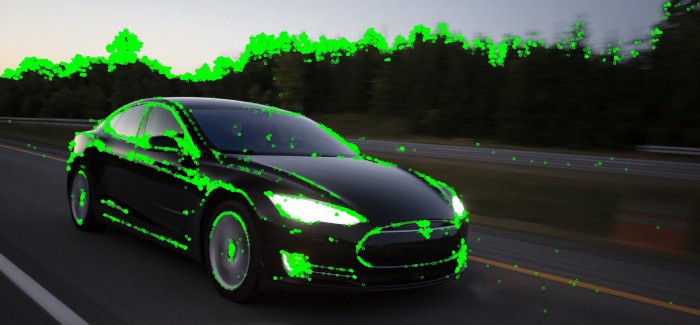
\includegraphics[width=0.7\linewidth]{images/recognition/kpMatch_tesla}
	\caption{The feature localization module applied to a Tesla. The key points are spread along the edges of the car and the background. Instead, the road has not, because the patter is often repeated, hence it is not reliable.}
	\label{fig:kpMatch_tesla}
\end{figure}
\begin{figure}[!h]
\centering
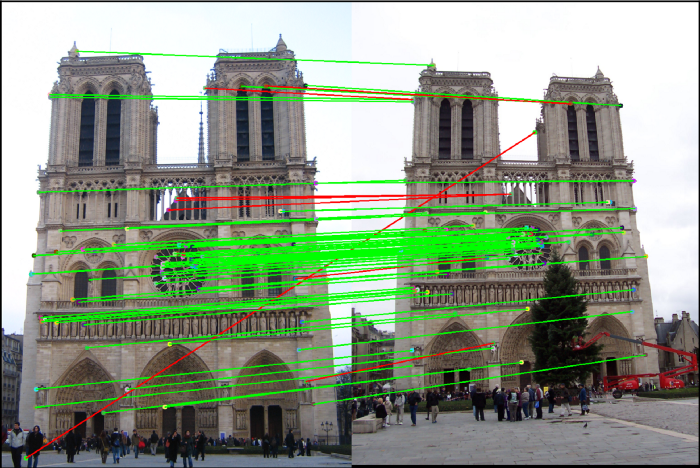
\includegraphics[width=0.7\linewidth]{images/recognition/kpMatch_notreDame}
\caption{Two images of Notre Dame de Paris are aligned with the feature matcher. Since the image is very clear a lot of points are paired correctly (green lines), while a few of them are not (red lines).}
\label{fig:kpMatch_notreDame}
\end{figure}

\subsubsection*{Key points matching applied to people}
The initial idea was to apply the key point matching to people. The test were done on the \textbf{Market1501}\cite{market1501} and on the \textbf{PRID450 (Person Re-IDentification)}\cite{prid450} datasets that contains thousands of images of cropped people walking outdoors. The datasets are constructed with multiple shots of the same person on different moment and prospectives.\\
The idea has two big problems:
\begin{itemize}
	\item The images cropped around the people has a very low resolution. The result is that the details that could distinguish a person from another one cannot be visible, or better cannot be recognised.
	\item Humans present a high deformable-body, with a surface (clothes) that continuously change aspect. Instead, the key point matching is designed for a pattern that is repeated often and clearly. The consequence of this is a matching that works as if it were random.
\end{itemize}
In~\Cref{fig:kpMatch_samples} are shown some examples that visually demonstrate the unreliability of this technique applied to humans.

\begin{figure}[!h]
	\centering
	\begin{subfigure}[!h]{0.24\textwidth}
		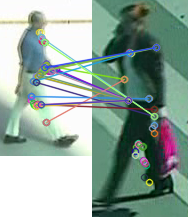
\includegraphics[width=\linewidth]{images/recognition/kpSample_aLotofMatches2}
	\end{subfigure}
	\begin{subfigure}[!h]{0.24\textwidth}
		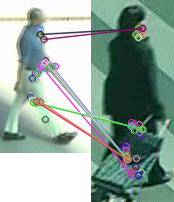
\includegraphics[width=\linewidth]{images/recognition/kpSample_object2}
	\end{subfigure}
	\begin{subfigure}[!h]{0.24\textwidth}
		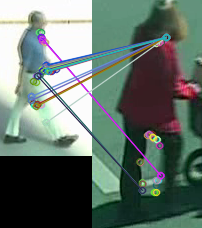
\includegraphics[width=\linewidth]{images/recognition/kpSample_falsePositive}
	\end{subfigure}
	\begin{subfigure}[!h]{0.24\textwidth}
		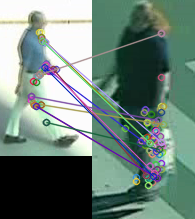
\includegraphics[width=\linewidth]{images/recognition/kpSample_object}
	\end{subfigure}
	%
	\begin{subfigure}[!h]{0.24\textwidth}
		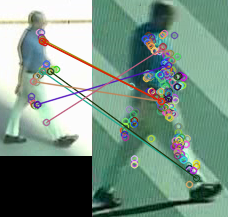
\includegraphics[width=\linewidth]{images/recognition/kpSample_samePerson}
	\end{subfigure}
	\begin{subfigure}[!h]{0.24\textwidth}
		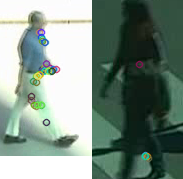
\includegraphics[width=\linewidth]{images/recognition/kpSample_noMatch}
	\end{subfigure}
	\begin{subfigure}[!h]{0.24\textwidth}
		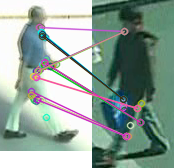
\includegraphics[width=\linewidth]{images/recognition/kpSample_aLotofMatches}
	\end{subfigure}
	\begin{subfigure}[!h]{0.24\textwidth}
		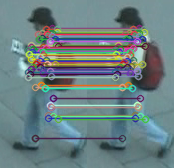
\includegraphics[width=\linewidth]{images/recognition/kpSample_self}
	\end{subfigure}
	\caption{Some matching samples show that key point matching easily fails under these conditions. There are multiple wrong aspects: people that present no key points, objects such as bags that have plenty of features, matching that connects completely different parts of the body like shoulders with legs. Even with the same subject with almost the same position (bottom-left images), the algorithm fails with most of the points. The exception is the bottom-right image that has a perfect matching, but the two pictures are exactly the same one. So it is not a reliable test.}
	\label{fig:kpMatch_samples}
\end{figure}


\section{KNN (K-Nearest Neighbors) with images into N-dimensional space}\label{sec:knn} \label{sec:classifiers}







googleNet, ResNet50, \cite{ssp_reID}